%%%%%%%%%%%%%%%%%%%%%%%%%%%%%%%%%%%%%%%%%%%%%%%%%%%%%%%%%%%%%%%%%%%%%%%%%%%%%%%%%%%%%%%%%%%%%%%%%%%
% Chapter 3 -> Methods
% Author: Eduardo G Gusmao
%%%%%%%%%%%%%%%%%%%%%%%%%%%%%%%%%%%%%%%%%%%%%%%%%%%%%%%%%%%%%%%%%%%%%%%%%%%%%%%%%%%%%%%%%%%%%%%%%%%
\chapter{Methods}
\label{cha:methods}

\graphicspath{{chapter3/figs/}}

% Chapter overview
In this chapter we describe the computational footprinting framework we devised to address the problem of active transcription factor binding site (TFBS) identification. Here, we exclusively present and formalize our novel computational footprinting approach. Method parameterization and execution details of our and other methods will be made in the next chapter.

% Methodological framework
Our methodological framework is divided into two main parts:
\begin{itemize}
\item In the first part, we discuss the input data processing (Section~\ref{sec:input.signal.processing}). We use data from next-generation sequencing (NGS) open chromatin experiments which gives information regarding the chromatin structure, allowing an accurate search for patterns of active TFBSs. In this first part we describe all steps involved in the generation of DNase-seq and ChIP-seq signals from the aligned reads and treatment of these signals through several steps which aim at reducing bias and normalizing such genomic signals.
\item In the second part, we define the novel method to identify footprints (i.e. putative active TFBSs) using the processed signals (Section~\ref{sec:computational.footprinting.hmm}). Such method is based on the probabilistic framework of hidden Markov models (HMMs).
\end{itemize}

% Implementation
Furthermore, we describe some details of the computational implementation of the methods described in this chapter (Section~\ref{sec:implementation}). Finally, we close this chapter with a few concluding remarks on the methodology choice and novelty of our approach (Section~\ref{sec:discussion.3}).

%%%%%%%%%%%%%%%%%%%%%%%%%%%%%%%%%%%%%%%%%%%%%%%%%%%%%%%%%%%%%%%%%%%%%
% Section: Input Signal Processing
%%%%%%%%%%%%%%%%%%%%%%%%%%%%%%%%%%%%%%%%%%%%%%%%%%%%%%%%%%%%%%%%%%%%%
\section{Input Signal Processing}
\label{sec:input.signal.processing}

% Introduction
As mentioned in Section~\ref{sec:current.challenges}, biological data from open chromatin NGS-based experiments, such DNase-seq and ChIP-seq are affected by biases and noises intrinsic to the experimental protocol. Therefore, a number of data processing steps are performed to assuage these biases and noises and also to prepare the data for our computational footprinting method.

% Data as aligned reads
The input data processing pipeline is schematically represented in Figure~\ref{fig:gusmao_signal_pipeline}. In this thesis, we use DNase-seq and histone modification ChIP-seq data as the input for our computational footprinting framework. With such data we are able to identify patterns of active transcription factor binding by analyzing the regions in the genome which are both open and protected against DNase I digestion (Section~\ref{sec:chromatin.based.method}). Our method receives as input the DNase-seq and histone modification ChIP-seq aligned reads (Figure~\ref{fig:gusmao_signal_pipeline}a).

\begin{figure}[h!]
\centering
\vspace{1.2cm}
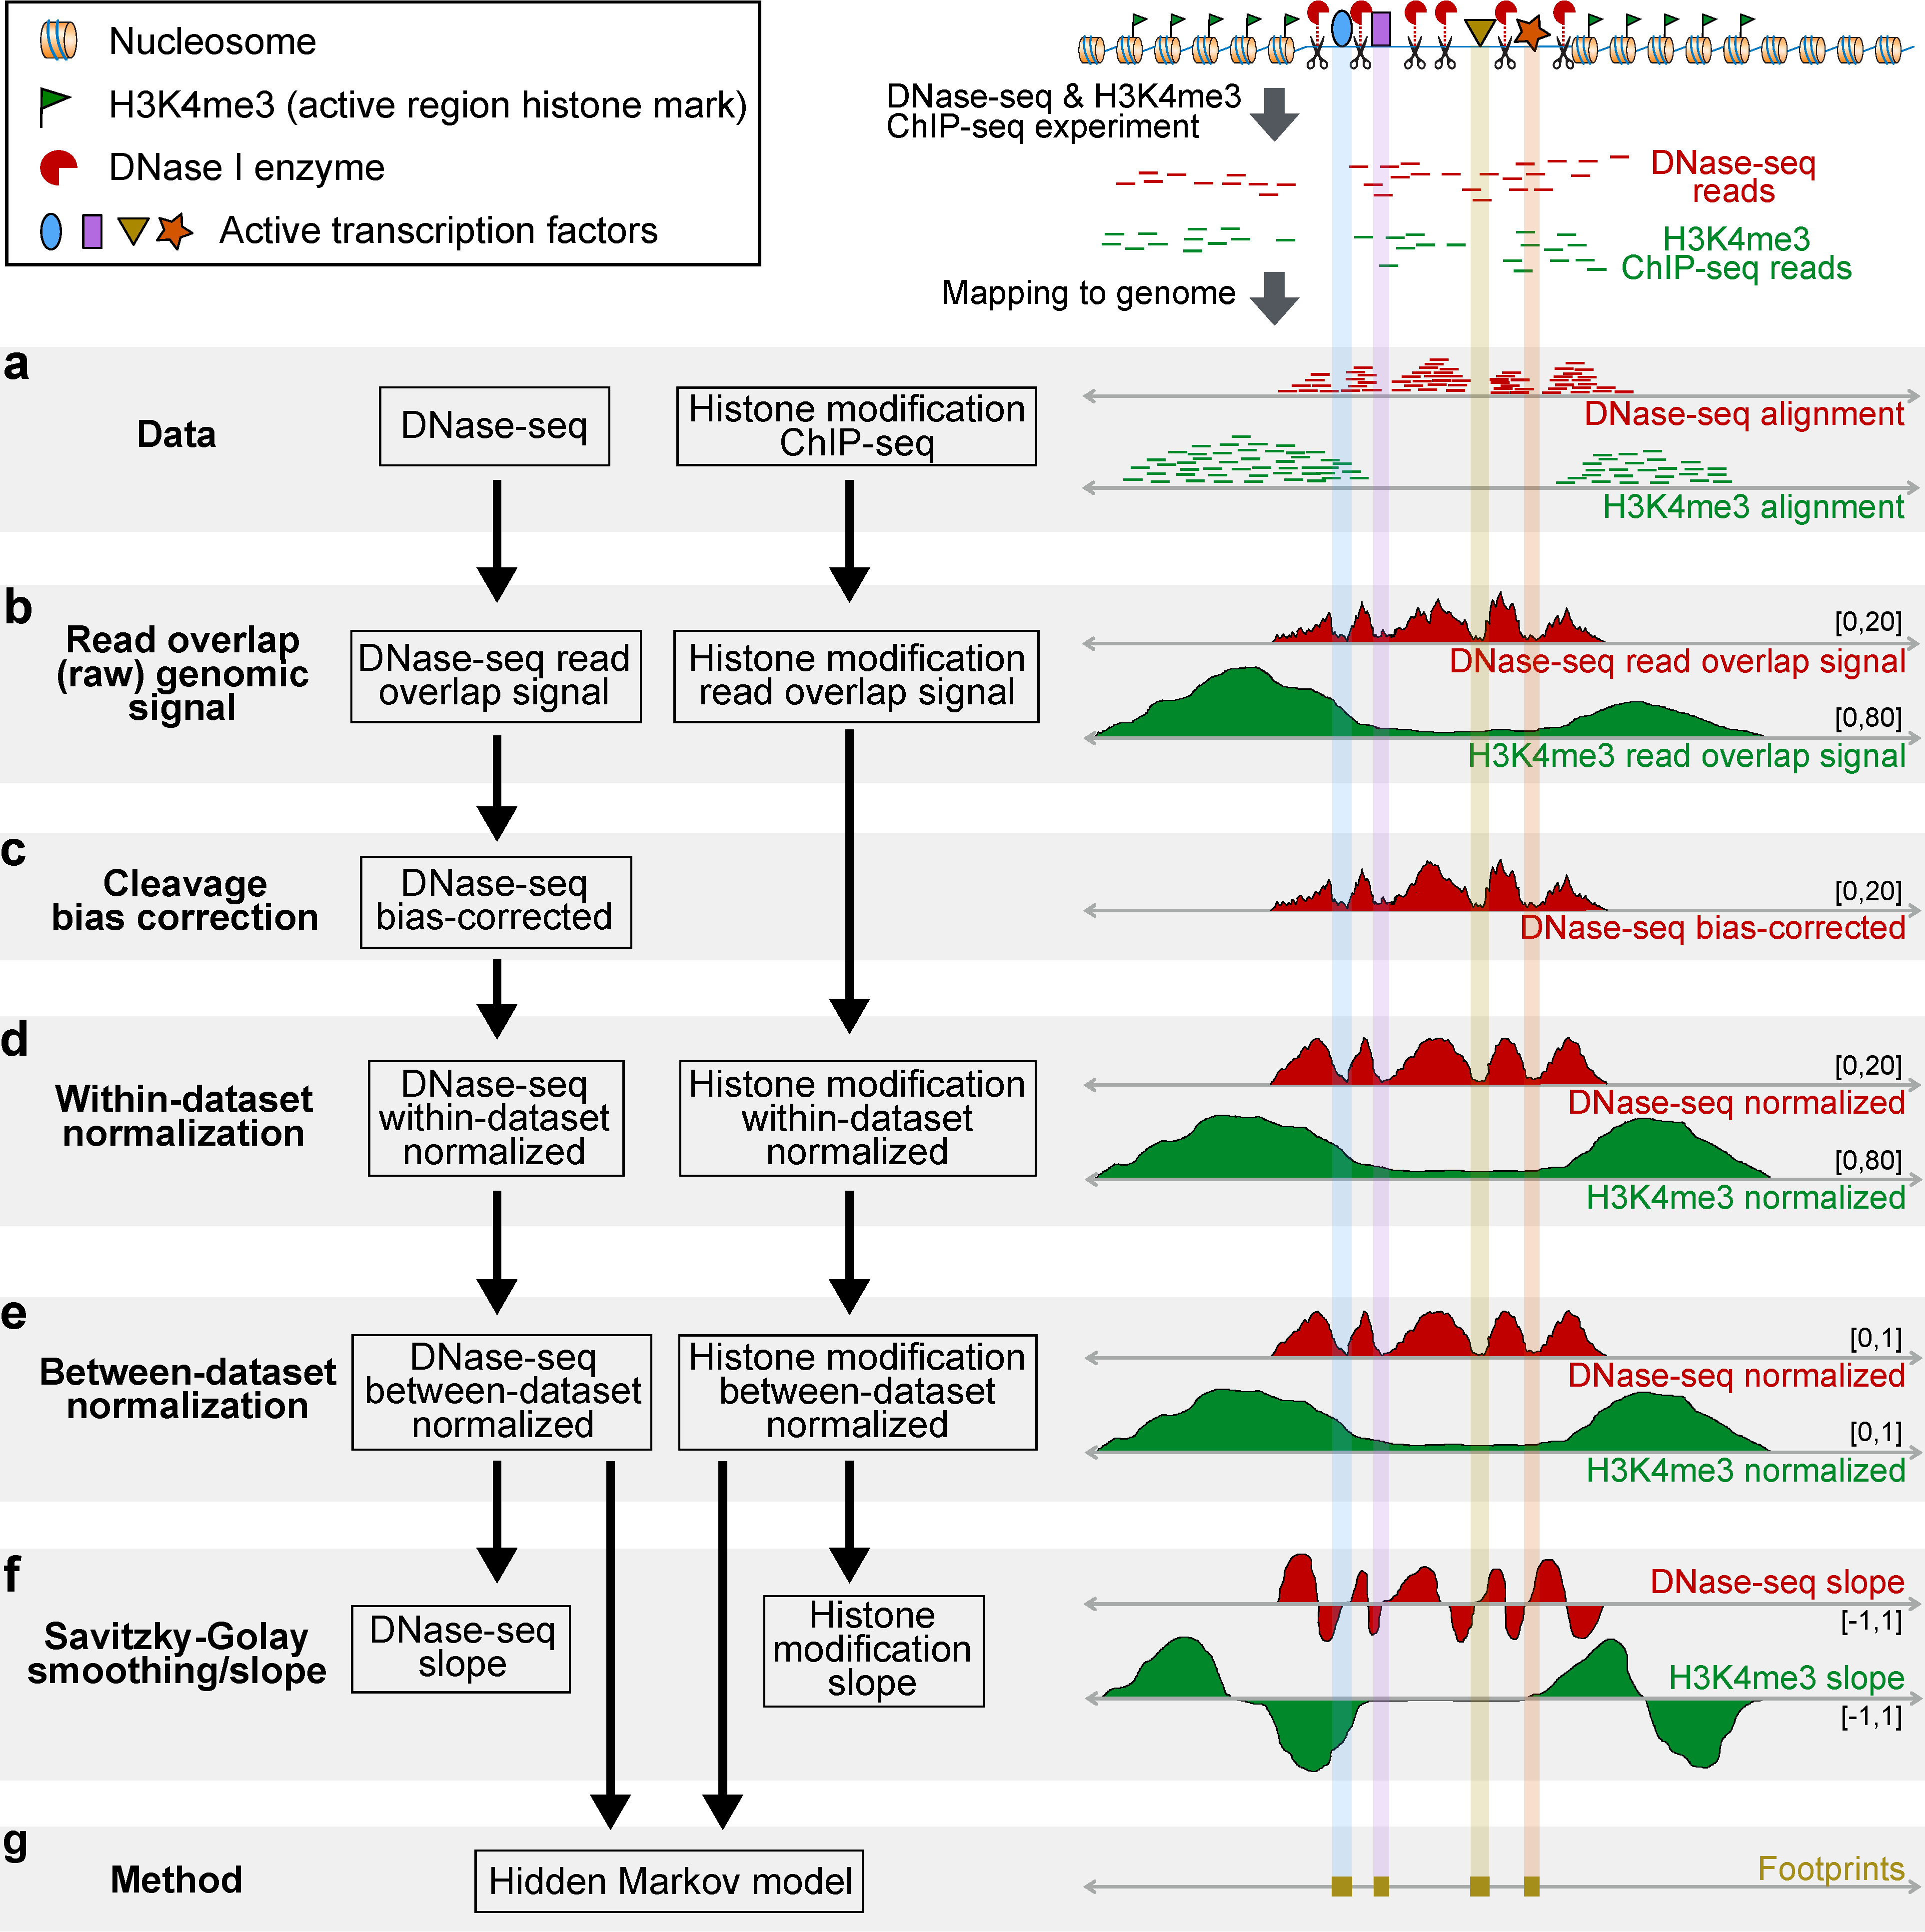
\includegraphics[width=0.99\textwidth]{gusmao_signal_pipeline}
\vspace{0.1cm}
\caption[Overview of input signal processing framework]{\textbf{Overview of input signal processing framework.} This figure provides a schematic representation of the input signal processing pipeline (left panels) and visual examples of the effects of these processing steps (right panels). The interval in each genomic signal represents the data scale. (\textbf{a}) We obtained DNase-seq (always represented in red) and histone modification data (always represented in green) as aligned reads. (\textbf{b}) A read overlap (raw) signal is generated by counting the number of overlapping aligned reads. (\textbf{c}) The DNase-seq signal needs to be corrected for sequence cleavage bias. (\textbf{d}) Then, both read overlap histone modification ChIP-seq and sequence cleavage bias-corrected DNase-seq signals are normalized using a within-dataset approach. This decreases the magnitude differences between the signal peaks within each dataset, while preserving the scale of the data. (\textbf{e}) Afterwards, both signals undergo a between-dataset normalization procedure to allow all datasets to be within the same scale of $[0, 1]$. (\textbf{f}) The slope of both signals are calculated using the Savitzky-Golay smoothing filter and differentiation methodology. (\textbf{g}) The DNase-seq and histone modification normalized and slope signals are the input for our computational footprinting method.}
\label{fig:gusmao_signal_pipeline}
\end{figure}

% Count and bias correction
Given the aligned reads, we create genomic signals by counting the overlap between these reads at every genomic coordinate (base pair; bp). This step, which is exemplified in Figure~\ref{fig:gusmao_signal_pipeline}b, is formally shown in Section~\ref{sec:read.overlap.signal}. We refer to this signal as read overlap (raw) genomic signal. The read overlap DNase-seq genomic signal is affected by the DNase-seq sequence cleavage bias. Such bias stems from the fact that the DNase I enzyme prefers to bind to, and cleave, certain genomic sequences. Given that, we perform a DNase-seq sequence cleavage bias correction. The DNase-seq sequence cleavage bias correction, exemplified in Figure~\ref{fig:gusmao_signal_pipeline}c, is thoroughly defined in Section~\ref{sec:dnaseseq.sequence.cleavage.bias}. This step performs local corrections in the DNase-seq signal while preserving signal scale, magnitude and shape.

% Normalization
Both bias-corrected DNase-seq and read overlap histone modification ChIP-seq signals have different magnitude throughout the genome, i.e. the height of the peaks within each of these signals vary greatly in distinct genomic regions. In order to normalize these signals while preserving the signal scale and shape, we perform a within-dataset (local) normalization procedure (Section~\ref{sec:withindataset.normalization}). The effect of such normalization procedure, as seen on Figure~\ref{fig:gusmao_signal_pipeline}d, is the decrease in peak height variability between different genomic regions. Furthermore, since our goal is to integrate both DNase-seq and histone modification ChIP-seq signal, we perform a between-dataset (global) normalization approach (Section~\ref{sec:betweendataset.normalization}). As seen on Figure~\ref{fig:gusmao_signal_pipeline}e, such normalization approach brings these two different signals to the same data range, i.e. the data is fit into the interval $[0,1]$, without losing their underlying shape. After such normalization procedures, both signals will present less variability within and between datasets without enhancing background noise and without changes in the shape and duration of the signal's peaks.

% Slope
Our computational footprinting method uses the increase and decrease of the signals. Therefore, we also apply a method called Savitzky-Golay smoothing filter and differentiation to calculate the slope of the signal based on a certain window of data points (Section~\ref{sec:savitzkygolay.smoothing.slope}). We observe in Figure~\ref{fig:gusmao_signal_pipeline}f that such slope signal assumes high positive values when there is an increase in the genomic signal and a low negative value when there is a decrease in the genomic signal. The normalized and slope versions of the DNase-seq and histone modification ChIP-seq signals correspond to our computational footprinting method's input, as will be described in Section~\ref{sec:computational.footprinting.hmm}.

%%%%%%%%%%%%%%%%%%%%%%%%%%%%%%%%%%%%%%%%%%%%%%%%%%%%%%%%%%%%%%%%%%%%%
% Section: Read Overlap Signal
%%%%%%%%%%%%%%%%%%%%%%%%%%%%%%%%%%%%%%%%%%%%%%%%%%%%%%%%%%%%%%%%%%%%%
\subsection{Read Overlap Signal}
\label{sec:read.overlap.signal}

% Genome
NGS experiments, such as DNase-seq and ChIP-seq, provide multiple reads, i.e., short deoxyribonucleic acid (DNA) sequences that are aligned into the genome. Here we formally define the genome as a vector
\begin{equation}
  \label{eq:genome}
  \mathbf{g} = \langle {g}_{1}, \cdots, {g}_{n} \rangle,
\end{equation}
where $n$ equals the number of base pairs (coordinates) in the genome and each ${g}_{i} \in \{\text{A}, \text{C}, \text{G}, \text{T}\}$ represents a nucleotide. As described in Section~\ref{sec:basic.concepts.molecular.biology} the DNA has two strands, which we refer to as the forward and reverse strand. Throughout this thesis consider $\mathbf{g}$ as the forward strand. Strand differentiation will be mentioned only when this issue is important. Moreover, the reverse strand can be inferred from the forward strand since each nucleotide pairs with a specific matching nucleotide. We denote as $\mathbf{g}[u..v]$ a substring of $\mathbf{g}$ from the genomic coordinate $u$ to $v$ for all $u \leq v$, including both within the interval. Therefore, $\mathbf{g}[u..v]$ has total length $u-v+1$.

% Genomic region and genomic region set
Furthermore, we refer to the term ``genomic region'' to denote an interval from a particular genomic coordinate $u$ to another genomic coordinate $v$. The genomic regions, as the genomic DNA substrings, have both initial ($u$) and final ($v$) positions within the interval and $u \leq v$ for all intervals, which have length $u-v+1$. A ``genomic region set'' is a collection of genomic regions, which are be represented as $R = \{ {r}_{1}, \cdots, {r}_{m} \}$.

% NGS experiments
We represent the reads obtained from any open chromatin NGS-based experiment, which are aligned into a genome $\mathbf{g}$, as a genomic regions set. Let $ R = \{ {r}_{1}, \cdots, {r}_{m} \}$ be the set of $m$ genomic regions representing the reads from a particular NGS experiment aligned in $\mathbf{g}$. In this case, each ${r}_{i} = [u, v, s]$ represents a triple, where $u$ is the coordinate in $\mathbf{g}$ where the aligned read starts, $v$ is the coordinate in $\mathbf{g}$ where the aligned read ends and $s \in \{\Plus, \Minus\}$ corresponds to the DNA strand in which the read was aligned to ($\Plus$ represents the forward strand, while $\Minus$ represents the reverse strand).

% Genomic signal
With such a set $R$ of genomic regions representing the aligned reads we are able to create a genomic signal $\mathbf{x}$, defined as a vector
\begin{equation}
  \label{eq:raw.signal}
  \mathbf{x} = \langle {x}_{1}, \cdots, {x}_{n} \rangle,
\end{equation}
by evaluating the overlap between the aligned reads $R$. Each $x_i \in {\mathbb{N}}^{0}$ represents the number of reads in $R$ that overlapped at the genomic position $i$.

% Extension
However, as previously discussed in Section~\ref{sec:ngs.methods}, only the first base pairs of the DNA fragments obtained from the biological experiments are sequenced by NGS techniques. We are interested in evaluating the overlap of different aligned genomic regions (representing the aligned reads) for different biological experiments (DNase-seq and ChIP-seq). Consequently, we first define a mapping function, which maps a particular read interval to a genomic region based on an extension parameter $\eta$. Such function is written as
\begin{equation}
  \label{eq:raw.signal.extension}
  {f}^{\text{ext}}({r}_{i}, \eta) = {f}^{\text{ext}}([u, v, s], \eta) =
  \begin{cases}
    [u,u+\eta] & \text{if } s = \Plus \\
    [v-\eta,v] & \text{ else.}
  \end{cases}
\end{equation}

% Genomic signal as overlap
With the extension function, we are able to define the overlap signal ($\mathbf{x}$) as
\begin{equation}
  \label{eq:raw.signal.overlap}
  {x}_{i} = \sum_{{r}_{j} \in R} \mathbf{1}\left( i \in {f}^{\text{ext}}({r}_{j}, \eta) \right),
\end{equation}
where ${\mathbf{1}}(\cdot)$ is an indicator function, which returns $1$ if its parameter proposition is true or $0$ otherwise.

% DNase-seq and ChIP-seq extension
The extension parameter used for the DNase-seq is $\eta = 1$ bp, since we are interested in the regions in which the DNase I enzyme nicked the DNA, i.e. the start of each read. The extension parameter used for ChIP-seq experiments is $\eta = 200$ bp. Such read size matches the average length of the DNA fragments retrieved during the chromatin immunoprecipitation procedure.

%%%%%%%%%%%%%%%%%%%%%%%%%%%%%%%%%%%%%%%%%%%%%%%%%%%%%%%%%%%%%%%%%%%%%
% Section: DNase-seq Sequence Cleavage Bias
%%%%%%%%%%%%%%%%%%%%%%%%%%%%%%%%%%%%%%%%%%%%%%%%%%%%%%%%%%%%%%%%%%%%%
\subsection{DNase-seq Sequence Cleavage Bias}
\label{sec:dnaseseq.sequence.cleavage.bias}

% Introduction
DNase-seq data was found to be affected by the DNase-seq sequence cleavage bias~\citep{he2014,meyer2014}. This happens because the DNase I enzyme has an intrinsic preference to bind to (and cleave) certain DNA sequences. In this section we describe our approach to estimate the DNase-seq sequence cleavage bias and to correct the DNase-seq signal for such bias.

%%%%%%%%%%%%%%%%%%%%%%%%%%%%%%%%%%%%%%%%%%%%%%%%%%%%%%%%%%%%%%%%%%%%%
% Section: Estimation of DNase-seq Sequence Cleavage Bias
%%%%%%%%%%%%%%%%%%%%%%%%%%%%%%%%%%%%%%%%%%%%%%%%%%%%%%%%%%%%%%%%%%%%%
\subsubsection{Estimation of DNase-seq Sequence Cleavage Bias}

% Introduction
The estimation of DNase-seq sequence cleavage bias is performed based on DNA sequence words of length $k$ ($k$-mers). Since we want to capture the DNase-seq sequence cleavage bias within particular regions enriched with DNase I activity, such bias estimation is performed in a set of genomic regions of interest $H = \{{h}_{1}, \cdots, {h}_{m}\}$. Our approach consists on measuring, within these genomic regions of interest: (1) the observed DNase I cleavage score for a $k$-mer $\mathbf{w}$, which corresponds to the number of DNase-seq cleavage hits centered on $\mathbf{w}$; and (2) the background DNase-seq cleavage score, which is defined by the total number of times $\mathbf{w}$ occurs. Then, the bias estimation is computed as the ratio between the observed and background cleavage scores. Such estimation is performed for all possible $k$-mers within the DNA alphabet $\{\text{A}, \text{C}, \text{G}, \text{T}\}$.

% Strand-specific
The process of estimation and correction of DNase-seq sequence cleavage bias is strand-specific, which means that we will consider the DNA sequences and signal generated separately for each DNA strand. However, for simplicity of notation, we will not explicitly denote strandedness in the equations.

% Observed cleavage score
For each possible $k$-mer $\mathbf{w}$, which is a string of length $k$ constructed with symbols from the DNA alphabet $\{\text{A}, \text{C}, \text{G}, \text{T}\}$, the observed cleavage score ${o}_{\mathbf{w}}$ is calculated, for a set of genomic regions of interest $H = \{h_1, \cdots, h_m\}$, as
\begin{equation}
  \label{eq:obscleav}
  {o}_{\mathbf{w}} = 1 + \sum_{i=1}^{m} \sum_{j \in h_i} {x}_{j} \mathbf{1}\left( \mathbf{g}[j-\frac{k}{2} .. j+\frac{k}{2}] = \mathbf{w}\right).
\end{equation}

% Background cleavage score
Similarly, the background cleavage score ${h}_{\mathbf{w}}$ is calculated as
\begin{equation}
  \label{eq:backcleav}
  {h}_{\mathbf{w}} = 1 + \sum_{i=1}^{m} \sum_{j \in h_i} \mathbf{1} \left( \mathbf{g}[j-\frac{k}{2} .. j+\frac{k}{2}] = \mathbf{w}\right).
\end{equation}

% Cleavage bias score
Finally, the estimated cleavage bias ${b}_{i}$ for a genomic position $k+1 \leq i \leq m-k+1$, given that $\mathbf{w}=\mathbf{g}[i-\frac{k}{2}..i+\frac{k}{2}]$, is calculated as
\begin{equation}
  \label{eq:cleavbias}
  {b}_{i} = \frac{{o}_{\mathbf{w}}}{{h}_{\mathbf{w}}}.
\end{equation}

% Conclusion
The estimated genomic bias signal point ${b}_{i}$ represents how many times the $k$-mer sequence $\mathbf{g}[i-\frac{k}{2}..i+\frac{k}{2}+1]$ was cleaved by the DNase I enzyme in comparison to its total occurrence in the set of regions of interest $H$.

%%%%%%%%%%%%%%%%%%%%%%%%%%%%%%%%%%%%%%%%%%%%%%%%%%%%%%%%%%%%%%%%%%%%%
% Section: Correction of DNase-seq Sequence Cleavage Bias
%%%%%%%%%%%%%%%%%%%%%%%%%%%%%%%%%%%%%%%%%%%%%%%%%%%%%%%%%%%%%%%%%%%%%
\subsubsection{Correction of DNase-seq Sequence Cleavage Bias}

% Introduction
The DNase-seq sequence cleavage bias correction is performed on smoothed versions of both read overlap DNase-seq ($\mathbf{x}$) and bias score $\mathbf{b}$ signals. The rationale is that we want to avoid dramatic signal changes generated within nucleotide-resolution bias signals.

% Smoothed DNase-seq signal
First, we create a smoothed DNase-seq signal $\hat{\mathbf{x}}$ using a $50$ bp window, which is written as
\begin{equation}
  \label{eq:smoothed.raw.dnase}
  {\hat{x}}_{i} = \frac{{x}_{j}}{\sum_{j=i-25}^{i+24} {x}_{j}}.
\end{equation}

% Smoothed bias score signal
Then, we create a smoothed bias score signal $\hat{\mathbf{b}}$ using the same $50$ bp window as for the smoothed DNase-seq signal, which is denoted as
\begin{equation}
  \label{eq:smoothed.bias.signal}
  {\hat{b}}_{i} = \frac{{b}_{j}}{\sum_{j=i-25}^{i+24} {b}_{j}}.
\end{equation}

% Bias-correction signal
With $\hat{\mathbf{x}}$ and $\hat{\mathbf{b}}$, we are able to calculate a signal of bias-correction factors $\mathbf{c}$ as
\begin{equation}
  \label{eq:bias.corr}
  {c}_{i} = {\hat{x}}_{i} {\hat{b}}_{i}.
\end{equation}

% Pre-processed DNase-seq bias-corrected signal
The pre-processed bias-corrected DNase-seq genomic signal ($\hat{\mathbf{x}}^{\text{bc}}$) is obtained by applying
\begin{equation}
  \label{eq:pre.bias.corr.signal}
  {\hat{x}}_{i}^{\text{bc}} = \log({x}_{i} + 1) - \log({c}_{i} + 1).
\end{equation}

% Global minumum
The pre-processed bias-corrected DNase-seq signal generated by Equation~\ref{eq:pre.bias.corr.signal} may include negative values. Since a few posterior statistical analyses required a signal consisting only of positive values, we have shifted the entire signal by adding the global (genomic) minimum value. The global minimum value $\zeta$ in the pre-processed bias-corrected DNase-seq signal is denoted as
\begin{equation}
  \label{eq:pre.dnase.corr.min}
  \zeta = \min_{i = 1, \cdots, n} {\hat{x}}_{i}^{\text{bc}}.
\end{equation}

% DNase-seq bias-corrected signal
The final DNase-seq bias-corrected signal $\mathbf{x}^{\text{bc}}$ is calculated by summing the pre-processed bias-corrected DNase-seq genomic signal ($\hat{\mathbf{x}}^{\text{bc}}$) and the absolute global minimum value ($\zeta$). Such summation is simply defined as
\begin{equation}
  \label{eq:bias.corr.signal}
  {x}_{i}^{\text{bc}} = {\hat{x}}_{i}^{\text{bc}} + |\zeta| .
\end{equation}
where $|\cdot|$ represents the absolute value of a number.

%%%%%%%%%%%%%%%%%%%%%%%%%%%%%%%%%%%%%%%%%%%%%%%%%%%%%%%%%%%%%%%%%%%%%
% Section: Within-Dataset Normalization
%%%%%%%%%%%%%%%%%%%%%%%%%%%%%%%%%%%%%%%%%%%%%%%%%%%%%%%%%%%%%%%%%%%%%
\subsection{Within-Dataset Normalization}
\label{sec:withindataset.normalization}

% Introduction
The next pre-processing step is applied on both DNase-seq sequence bias-corrected signal and read overlap histone modification ChIP-seq signal. From this point further, DNA strand information is not relevant anymore because we disregard the underlying DNA sequence. We will denote both these signals (bias-corrected DNase-seq and read overlap histone modification ChIP-seq) here as $\mathbf{x}$ for simplicity. This procedure is applied separately on each genomic signal. The within-dataset normalization step aims to reduce the intrinsic variability present within DNase-seq or ChIP-seq data. Such variability arise from the multiple biological and computational protocol steps.

% Genome binning
First, the genome is partitioned into a set of non-overlapping bins ${Y} = \{ {y}_{1}, \cdots, {y}_{m} \}$, where each ${y}_{l}$ represents the interval $[((l-1) \cdot \iota )+1, l \cdot \iota]$ for a particular interval-length parameter $\iota$. Furthermore, we also create a genome partition of overlapping bins ${Z} = \{ {z}_{1}, \cdots, {z}_{m} \}$, where each ${z}_{l}$ represents the interval ${y}_{l}$ extended by $\iota/2$ on both sides.

% Within-dataset normalization
We are able to create a within-signal normalized signal by dividing the signal by non-zero signal averages~\citep{boyle2011} inside the proposed bins. For a given genomic signal entry $x_i$ at genomic coordinate $i$, such that $i \in {y}_{l}$, we apply
\begin{equation}
  \label{eq:signal.within.norm}
  {x}^{\text{norm1}}_{i} = \frac{{x}_{i}}{ 
                     \sum\limits_{j \in {z}_{l}} {x}_{j} \mathbf{1}({x}_{j} > 0)  \;\; \Big/  
                     \sum\limits_{j \in {z}_{l}} \mathbf{1}({x}_{j} > 0)
                     }.
\end{equation}

%%%%%%%%%%%%%%%%%%%%%%%%%%%%%%%%%%%%%%%%%%%%%%%%%%%%%%%%%%%%%%%%%%%%%
% Section: Between-Dataset Normalization
%%%%%%%%%%%%%%%%%%%%%%%%%%%%%%%%%%%%%%%%%%%%%%%%%%%%%%%%%%%%%%%%%%%%%
\subsection{Between-Dataset Normalization}
\label{sec:betweendataset.normalization}

% Introduction
After the within-dataset normalization, we perform a between-dataset normalization procedure to force values inside the interval $ [0,1] $ by fitting the within-dataset normalized signals into a logistic function~\citep{hon2009}.

% Between-dataset normalization - local approach
Let ${Y} = \{ {y}_{1}, \cdots, {y}_{m} \}$ and ${Z} = \{ {z}_{1}, \cdots, {z}_{m} \}$ be non-overlapping and overlapping genomic partitions, respectively, as described in Section~\ref{sec:withindataset.normalization}. For a given genomic signal entry $x_i$ at genomic coordinate $i$, such that $i \in {y}_{l}$, we apply
\begin{equation}
  \label{eq:signal.between.norm.local}
  {x}^{\text{norm2}}_{i} = \frac{1}{1+e^{{-({x}^{\text{norm1}}_{i}-{\varsigma}^{t}_{{z}_{l}})}/{\sigma}_{{z}_{l}}}},
\end{equation}
where ${\varsigma}^{t}_{{z}_{l}}$ is the $t^{\text{th}}$ percentile of the signal data points within the interval ${z}_{l}$ and $\sigma_{{z}_{l}}$ is the standard deviation of the signal data points within the interval ${z}_{l}$, given by
\begin{equation}
  \label{eq:signal.between.var.local}
  \sigma_{{z}_{l}} = \sqrt{ \frac{\sum_{j \in {z}_{l}} \left({x}^{\text{norm1}}_{j} - \mu_{{z}_{l}}\right)^2}{2\iota} },
\end{equation}
where $\mu_{{z}_{l}}$ is the mean of the signal data points within the interval ${z}_{l}$, given by
\begin{equation}
  \label{eq:signal.between.mean.local}
  \mu_{{z}_{l}} = \sum_{j \in {z}_{l}} \frac{{x}^{\text{norm1}}_{j}}{2\iota}.
\end{equation}

% Normalized signal
After the application of the within-dataset and between-dataset normalization procedures (for both DNase-seq and histone modification ChIP-seq), we consider the output as our ``normalized'' signal. For simplicity, we will denote such signal as $\mathbf{x}^{\text{norm}}$.

%%%%%%%%%%%%%%%%%%%%%%%%%%%%%%%%%%%%%%%%%%%%%%%%%%%%%%%%%%%%%%%%%%%%%
% Section: Savitzky-Golay Smoothing and Slope
%%%%%%%%%%%%%%%%%%%%%%%%%%%%%%%%%%%%%%%%%%%%%%%%%%%%%%%%%%%%%%%%%%%%%
\subsection{Savitzky-Golay Smoothing and Slope}
\label{sec:savitzkygolay.smoothing.slope}

% Introduction
Our computational footprinting method uses an additional signal, which indicates upward and downward trends in the normalized genomic signals. We will use the slope of the normalized signal to assess such information~\citep{boyle2011}. In order to estimate the slope of the genomic signals we apply a Savitzky-Golay smoothing filter followed by differentiation~\citep{madden1978,luo2005}.

% Savitzky-Golay smoothing and differentiation
The Savitzky-Golay smoothing filter and differentiation method consists of fitting the data into a polynomial, performing a convolution (based on a specific window length $\tau$) with a vector containing Savitzky-Golay coefficients~\citep{madden1978}.

% Savitzky-Golay convolution
Let an odd-number $\tau$ be a specific window length in which the smoothing is going to be performed. The Savitzky-Golay convolution is expressed as
\begin{equation}
  \label{eq:slope}
  {x}^{\text{slope}}_{i} = \sum\limits_{j=-\hat{\tau}}^{\hat{\tau}} {c}_{j+\hat{\tau}} {x}^{\text{norm}}_{i+j},
\end{equation}
where $\hat{\tau}=\frac{\tau-1}{2}$ and $\mathbf{c}$ is the vector of Savitzky-Golay coefficients.

% Savitzky-Golay coefficients
The derivation of the Savitzky-Golay coefficients is performed using an analytic solution that enables the smoothing and differentiation within the same convolution depicted in Equation~\ref{eq:slope}. First, a polynomial will be fitted by linear least squares to a set of $\tau$ adjacent data points. These are the same data points within the window of the convolution represented in Equation~\ref{eq:slope}. Then, let $\mathbf{z}$ be a variable which represents the index of the equally-spaced convolution, i.e. $\mathbf{z} = \{ {z}_{1}, {z}_{2}, \cdots, {z}_{\tau} \} = \{ -\hat{\tau}, \cdots, 0, \cdots, \hat{\tau}\}$. The fitted polynomial of degree $\tau$ is described as
\begin{equation}
  \label{eq:sg.polynomial}
  Y = {c}_{0} + {c}_{1}{z} + {c}_{2}{z}^{2} + {c}_{\tau}{z}^{\tau}.
\end{equation}

% Jacobian matrix
The coefficients $c_i$ are obtained by solving the linear square's normal equations
\begin{equation}
  \label{eq:savitzky.golay.coeff}
  \mathbf{c} = {\left( \mathbf{J}^{\intercal} \mathbf{J} \right)}^{-1} \mathbf{J}^{\intercal} \mathbf{\hat{x}},
\end{equation}
where $\mathbf{\hat{x}} $ is the vector of signals within the current convolution window of length $\tau$ (Equation~\ref{eq:slope}), and the  $i^{\text{th}}$ row of the Jacobian matrix $\mathbf{J}$, denoted as
\begin{equation}
  \label{eq:savitzky.golay.jacob}
  \frac{\partial \mathbf{\hat{x}} }{\partial \mathbf{c}},
\end{equation}
has values $ \langle 1, {z}_{i}, {z}_{i}^{2}, \cdots, {z}_{i}^{\tau} \rangle$.

% Full derivation
For the full linear squares derivation of the Savitzky-Golay coefficients and more details on the effects of such smoothing filter, please refer to~\cite{luo2005}.

%%%%%%%%%%%%%%%%%%%%%%%%%%%%%%%%%%%%%%%%%%%%%%%%%%%%%%%%%%%%%%%%%%%%%
% Section: Computational Footprinting with Hidden Markov Models
%%%%%%%%%%%%%%%%%%%%%%%%%%%%%%%%%%%%%%%%%%%%%%%%%%%%%%%%%%%%%%%%%%%%%
\section{Computational Footprinting with Hidden Markov Models}
\label{sec:computational.footprinting.hmm}

% Introductions
In order to detect footprints in genomic signals of the DNase-seq and histone modification ChIP-seq experiments we need a technique which is able to segment the genome from a multidimensional input. The grammar of active TFBSs shows a clear sequential pattern with regard to the intensities of the DNase-seq and histone modification signals. However, the length of each of these pattern's segment, i.e. length of the background regions (with no detectable signals), the length of histone modification or DNase-seq peaks and the duration of the footprints are diverse. Furthermore, segmented regions might present a similar level of the signals. For instance, both the background genomic regions and footprint genomic regions, which should definitely be separated by the computational footprinting segmentation method, have the same signal landscape, i.e. low (close to zero) signals of both DNase-seq and histone modification ChIP-seq signals. The difference between these regions is that the footprint happen within two peaks of DNase-seq signals, which happen within two peaks of active histone modification signals. Given these remarks, an obvious choice for such a segmentation task are hidden Markov models (HMMs). HMM is a computational technique based on Markov stochastic processes. Such computational model is defined thoroughly in Section~\ref{sec:multivariate.continuous.hmm}.

% Computational footprinting with HMMs
After defining the HMMs, we proceed to discuss how this probabilistic model is used to segment the genome in the context of the identification of active TFBSs. Figure~\ref{fig:gusmao_method_pipeline} shows a schematic pipeline of our computational footprinting framework using HMMs. First, we define a number of different model topologies based on the grammar of active TFBSs and on remarks made by recent studies on the heterogeneity of such grammar (Section~\ref{sec:hmm.topology}). The different HMM topologies take different input signals, which can be normalized and/or slope versions of the DNase-seq (Figure~\ref{fig:gusmao_method_pipeline}a) and histone modification ChIP-seq (Figure~\ref{fig:gusmao_method_pipeline}b) signals. The HMM topologies used in this thesis are stated in Figure~\ref{fig:gusmao_method_pipeline}c. Next, we define how the model is  trained in a supervised manner, using annotation of known TFBSs and a maximum-likelihood probability approach (Section~\ref{sec:hmm.training}; Figure~\ref{fig:gusmao_method_pipeline}d). Finally, the DNase-seq and histone modification ChIP-seq data are used as input for the trained HMMs to make predictions of active TFBSs. To accomplish such a task, we use the Viterbi algorithm (Section~\ref{sec:hmm.decoding}; Figure~\ref{fig:gusmao_method_pipeline}e).

% Figure - Computational footprinting framework
\begin{figure}[h!]
\centering
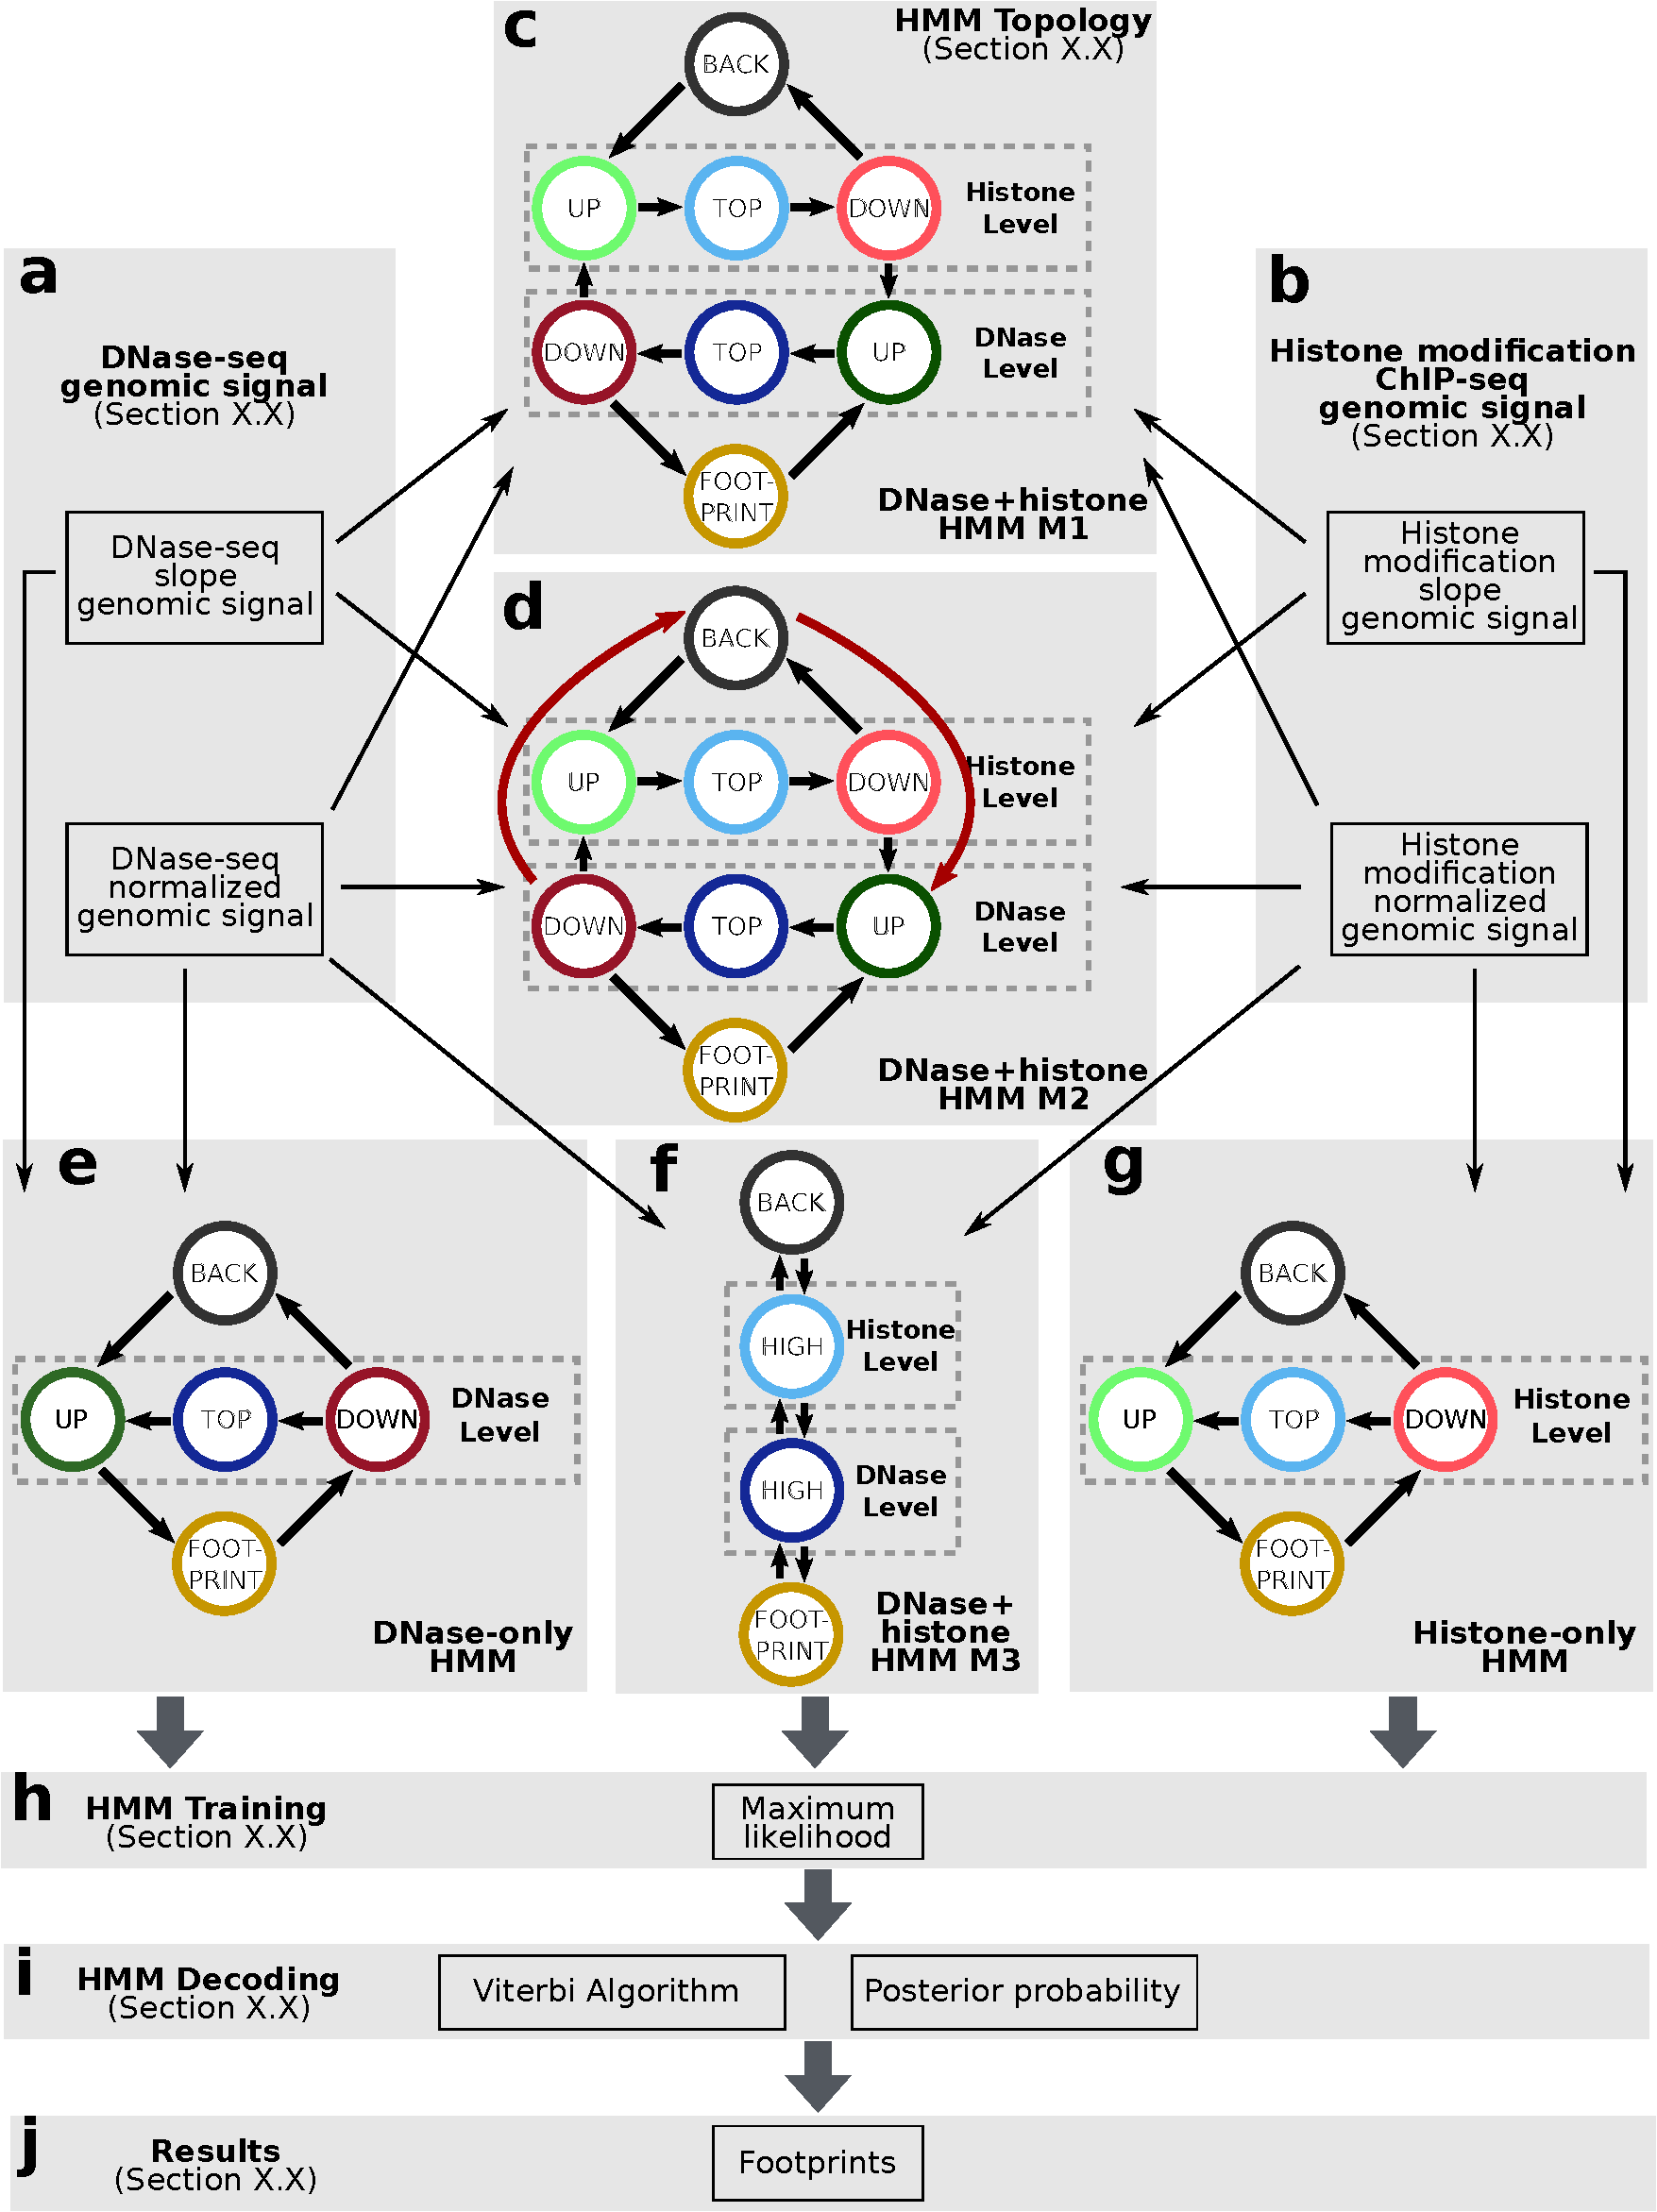
\includegraphics[width=0.87\textwidth]{gusmao_method_pipeline}
\caption[Computational footprinting framework]{\textbf{Computational footprinting framework.} Graphical representation of the computational footprinting method pipeline. (\textbf{a},\textbf{b}) Our computational footprinting method receives as input normalized and/or slope signals of DNase-seq and/or histone modification ChIP-seq. (\textbf{c}) Different HMM topologies were used. Such HMM topologies take different types of input data. (\textbf{d}) All HMMs are trained using the supervised maximum likelihood method. (\textbf{e}) We use the Viterbi algorithm to apply the HMM in the genomic signal and predict footprints. (\textbf{f}) The final footprints represent our predictions of putative active TFBSs.}
\label{fig:gusmao_method_pipeline}
\end{figure}

%%%%%%%%%%%%%%%%%%%%%%%%%%%%%%%%%%%%%%%%%%%%%%%%%%%%%%%%%%%%%%%%%%%%%
% Section: Multivariate Continuous HMM
%%%%%%%%%%%%%%%%%%%%%%%%%%%%%%%%%%%%%%%%%%%%%%%%%%%%%%%%%%%%%%%%%%%%%
\subsection{Multivariate Continuous HMM}
\label{sec:multivariate.continuous.hmm}

% Introduction
Markov chains are probabilistic models composed of a collection of states and transitions between these states~\citep{rabiner1989}. These transitions correspond to the probability of changing between states. The HMMs follow the same baseline idea, however they also contain within their model an unknown sequence of states associated to each input symbol~\citep{rabiner1989,durbin1998}. In this section we formalize the concept of HMMs.

% Parameters
First, we define the input data for our HMM as a matrix
\begin{equation}
  \label{eq:hmm.input.data}
  \mathbf{X} = \{x_{ij}\}^{d \times n}
\end{equation}
of $d$ observed multivariate continuous genomic signals, each of which has length $n$. For a given multivariate observation $\langle \mathbf{{x}_{\cdot 1}}, \cdots, \mathbf{{x}_{\cdot t}}, \cdots, \mathbf{{x}_{\cdot n}} \rangle$ from $\mathbf{X}$, we have a corresponding hidden sequence path $\mathbf{q} = \langle q_1, \cdots, q_t, \cdots, q_n \rangle$, where $ q_t \in W = \{1, \cdots, w\} $ represents the state emitting the vector $ {\mathbf{x}}_{\cdot t} $ at the $t^{\text{th}}$ genomic position and $w$ is the total number of states given a particular HMM topology.

% Independence assumptions
HMMs have two independence assumptions~\citep{rabiner1989}. The first assumption is that the probability to reach state $t$ depends only on the previous state $t-1$
\begin{equation}
  \label{eq:hmm.indep.1}
  p(q_t | q_1, \cdots, q_{t-1}) = p(q_t | q_{t-1}),
\end{equation}
and the second assumption dictates that the probability density function of emitting an input vector $\mathbf{{x}_{\cdot t}}$ observed at state $t$, depends only on this current state
\begin{equation}
  \label{eq:hmm.indep.2}
  p(\mathbf{{x}_{\cdot t}} | q_1, \cdots, q_t) = p(\mathbf{{x}_{\cdot t}} | q_t).
\end{equation}

% HMM problems - intuition 1
Given the formalism previously defined, there are three general problems which can be addressed directly through computationally efficient implementations of HMMs~\citep{durbin1998}. Let $\Theta$ be the parameters of a HMM, we state these problems as:

\begin{center}
  \begin{tabular}{lp{.8\linewidth}}
    {\bf Problem 1} & Estimate the HMM parameters $ \Theta $ in order to maximize $p(\mathbf{X} | \Theta)$. \\[0.2cm]
    {\bf Problem 2} & Given an observed multivariate input $ \mathbf{X} $ and an HMM represented by the parameters $ \Theta $, find the sequence of hidden states $ \mathbf{q} $ which best explains the input given the HMM, i.e. that maximizes $ p\left( \mathbf{X}, \mathbf{q} | \Theta \right) $ . \\[0.2cm]
    {\bf Problem 3} & Given an observed multivariate input $ \mathbf{X} $ and an HMM represented by the parameters $ \Theta $, compute the probability of the input sequence given the HMM $p(\mathbf{X} | \Theta)$. \\[0.2cm]
  \end{tabular}
\end{center}

% HMM problems - intuition 2
The first problem regards the HMM parameter estimation, i.e. model training. This problem will be addressed in Section~\ref{sec:hmm.training}. The second and third problems represent our genomic segmentation methodology using the HMM states in order to predict active binding sites. These problems will be explored in Section~\ref{sec:hmm.decoding}. For a more thorough discussion, including proof of theorems, we refer to~\cite{rabiner1989,durbin1998,mitchell1997,bishop2006,duda2000}.

% HMM Parameters
The multivariate continuous HMM used to address the aforementioned problems is defined, in terms of its parameters, as
\begin{equation}
  \label{eq:hmm.theta}
  \Theta= \{\mathbf{A}, \mathbf{E}, \mathbf{s}\}.
\end{equation}

% Transitions
The parameter $\mathbf{A}$ represents the matrix which contains the probabilities of transitioning between the states of the HMM. We formalize this as
\begin{equation}
  \label{eq:hmm.a}
  \mathbf{A} = {\{a_{uv}\}}^{w \times w},
\end{equation}
where $a_{uv}$ represents the probability of transition from state $u$ to $v$, which is
\begin{equation}
  \label{eq:hmm.transition}
  a_{uv} = p(q_t = v | q_{t-1} = u).
\end{equation}

% Emission
The parameter $\mathbf{E}$ represents the vector of probability density functions which represent the emissions of symbols by the HMM. More formally,
\begin{equation}
  \label{eq:hmm.e}
  \mathbf{E} = \langle e_1(\mathbf{x}), \cdots, e_{w}(\mathbf{x}) \rangle,
\end{equation}
where each state $u$ has a probability $e_u(\mathbf{x})$ of emitting the vector symbol $ \mathbf{x} $. Such probability density function is represented by
\begin{equation}
  \label{eq:hmm.emission}
  e_u(\mathbf{x}) = p( \mathbf{{x}_{\cdot t}} | q_t = u).
\end{equation}

% Initial state probabilities
The parameter $\mathbf{s}$ represents the initial state transition probabilities. This is represented as a vector of probabilities
\begin{equation}
  \label{eq:hmm.initial}
  \mathbf{s} = \langle s_{1}, \cdots, s_{w} \rangle,
\end{equation}
where each $s_i$ represents the probability of starting in a particular state.

%%%%%%%%%%%%%%%%%%%%%%%%%%%%%%%%%%%%%%%%%%%%%%%%%%%%%%%%%%%%%%%%%%%%%
% Section: HMM Topology
%%%%%%%%%%%%%%%%%%%%%%%%%%%%%%%%%%%%%%%%%%%%%%%%%%%%%%%%%%%%%%%%%%%%%
\subsection{HMM Topology}
\label{sec:hmm.topology}

% Introduction
We refer to HMM topology as the number of states $w$ and the predefined possible transitions between these states ($a_{uv} > 0$). The mathematical modeling of a problem with HMMs require the knowledge of the problem in order to be able to create a meaningful HMM topology. We implemented a number of different HMM topologies, depicted in Figures~\ref{fig:gusmao_hmm_footprinting}--\ref{fig:gusmao_model5}. It is important to mention that all HMM states from all topologies have transitions to itself, which were omitted in all figures for simplicity. In this section we will define these topologies and discuss the rationale behind each topology choice. To enhance clarity, the HMM states will also be represented with labels using the {\tt UPPERCASE COURIER} font. Also, the HMM topologies' names will be represented using the \textsc{Small Capitals} font.

% DNase + Histone model -- Model 1
\subsubsection{\textsc{DNase + Histone Model}}

% Introduction
The \textsc{DNase + histone model} (Figure~\ref{fig:gusmao_hmm_footprinting}) represents the main topology from our method. It combines both DNase-seq and histone modification ChIP-seq in an HMM structure devised to recognize the grammar of active TFBSs described in Section~\ref{sec:chromatin.based.method}. The idea behind this topology is that we are going to model the depletion between two peaks of DNase-seq using DNase-specific states and we model the open chromatin region within the depletion between two peaks of histone modification ChIP-seq using histone-specific states. We shall refer to this as the \textsc{original DNase + histone model}.

% Figure - DNase + histone model topology and genomic segmentation
\begin{figure}[h!]
\centering
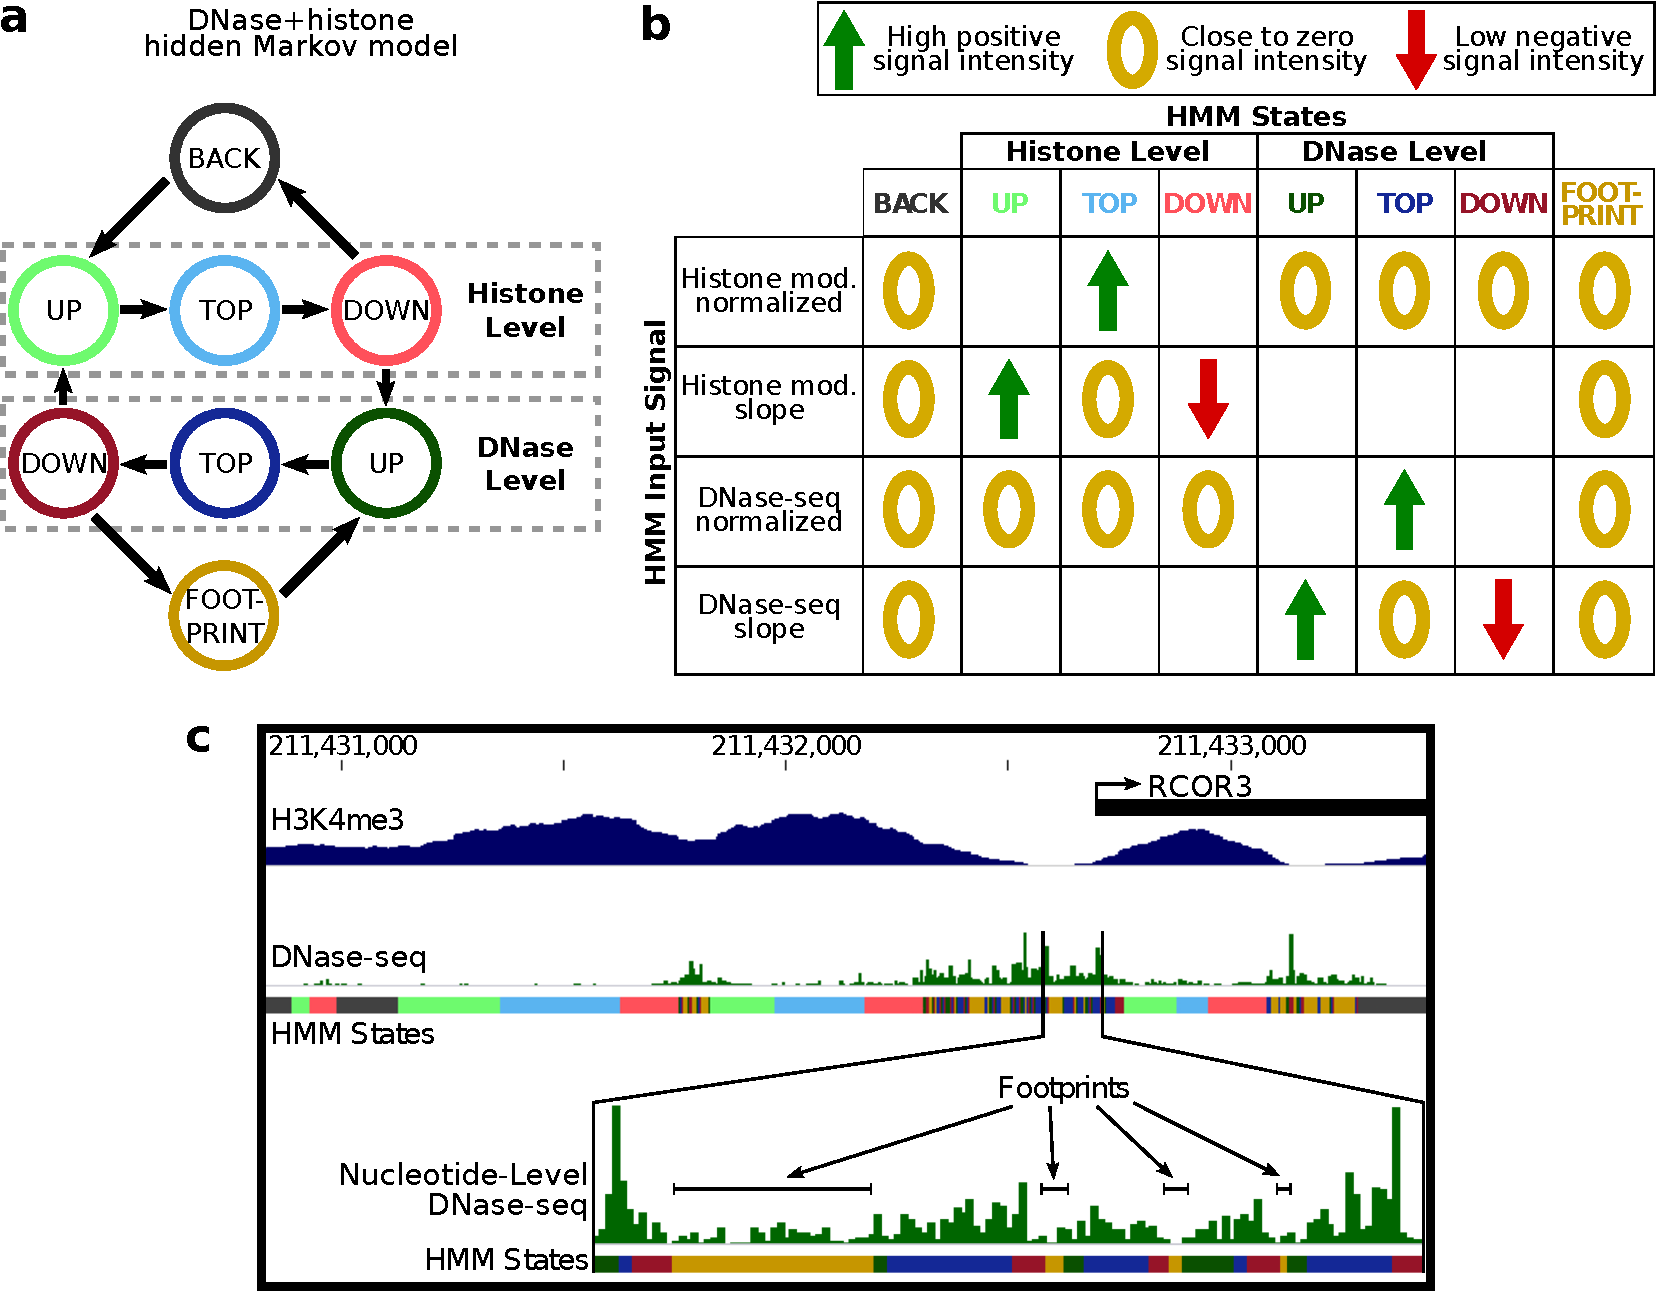
\includegraphics[width=0.99\textwidth]{gusmao_hmm_footprinting}
\caption[\textsc{DNase + Histone model} HMM topology and genomic segmentation]{\textbf{\textsc{DNase + Histone model} HMM topology and genomic segmentation.} (\textbf{a}) \textsc{DNase + Histone model} HMM topology. Each circle represents a labeled HMM state. Each arrow represents an allowed transition between states. Self-transitions exist in all states and were omitted for simplicity. (\textbf{b}) Summary of the normalized and slope versions of the DNase-seq and histone modification signals' intensities at each state of the \textsc{DNase + Histone model}. The blank cells within this table correspond to variable signal intensity between different input data and, although important for the final HMM decoding, are not prerequisite for the HMM's recognition of the grammar of TFBSs. (\textbf{c}) DNase-seq and H3K4me3 (ChIP-seq) signals around the promoter region of the RCOR3 gene. This region was annotated using the \textsc{DNase + Histone model}. The color code of the annotation matches the color code of the \textsc{DNase + Histone model} representation. We are able to observe several putative footprint predictions of varied sizes. \emph{Source:~\cite{gusmao2014}} (modified to fit thesis format and/or clarify key points).}
\label{fig:gusmao_hmm_footprinting}
\end{figure}

% Signal
In this topology, the input matrix $\mathbf{X}$ (Equation~\ref{eq:hmm.input.data}) consists on the normalized and slope versions of the DNase-seq and histone modification ChIP-seq signals. This input matrix can be represented as a vector of input signal vectors
\begin{equation}
  \label{eq:signal.m1}
  \mathbf{X} = \langle \quad \mathbf{x}^{\text{norm}}_{\text{dnase}} ,\quad \mathbf{x}^{\text{slope}}_{\text{dnase}} ,\quad \mathbf{x}^{\text{norm}}_{\text{histone}} ,\quad \mathbf{x}^{\text{slope}}_{\text{histone}} \quad \rangle .
\end{equation}

% Emission distribution is gaussian
The probability density function used for the emission probabilities ($\mathbf{E}$) correspond to a multivariate Gaussian (normal) density function with full covariance matrix. This is described as
\begin{equation}
  \label{eq:hmm.emission.gaussian}
  \begin{array}{lcl}
    p(\mathbf{{x}_{\cdot t}} | q_t = u) & = & 
    p(\mathbf{x_{\cdot t}}|{{\boldsymbol\mu}^{u}},{{\boldsymbol\Sigma}^{u}})\\[0.4em] & = &
    \frac{1}{ \sqrt{(2\pi)^{D} {| {{\boldsymbol\Sigma}^{u}} |}}}
    e^{-\frac{1}{2} (\mathbf{x_{\cdot t}}-{{\boldsymbol\mu}^{u}})^T ({{\boldsymbol\Sigma}^{u}})^{-1} (\mathbf{x_{\cdot t}}-{{\boldsymbol\mu}^{u}})}, \\
  \end{array}
\end{equation}
where ${{\boldsymbol\mu}^{u}}$ and ${{\boldsymbol\Sigma}^{u}}$ are, respectively, the $d$-dimensional mean vector and full covariance matrix of the emission probability density function at state $u$.

% Topology
Figure~\ref{fig:gusmao_hmm_footprinting}a shows a graphical representation of the \textsc{DNase + Histone model}. The first state ({\tt BACK}) corresponds to the ``background'' regions with low concentration of DNase-seq and histone modification ChIP-seq signals. The histone level states represent a peak in the histone modification ChIP-seq signal, recognizing an increase in the histone modification ChIP-seq signal based on high positive $x^{\text{slope}}_{\text{histone}}$ values ({\tt UP}), summit regions with $x^{\text{slope}}_{\text{histone}}$ values close to zero and high $x^{\text{norm}}_{\text{histone}}$ values ({\tt TOP}) and a decrease based on negative values of the $x^{\text{slope}}_{\text{histone}}$ signal ({\tt DOWN}). From the histone level {\tt DOWN} state, the model can either return to {\tt BACK} (isolated histone modification peaks without further DNase hypersensitivity sites) or continue to the DNase level {\tt UP} state. The DNase level states are equivalent to the histone level states, with the exception that the $x^{\text{norm}}_{\text{dnase}}$ and $x^{\text{slope}}_{\text{dnase}}$ signals are being recognized instead. From the DNase level {\tt DOWN} state, the model decides between returning to a region of higher histone modification ChIP-seq signals (histone level {\tt UP} state) and visiting the {\tt FOOTPRINT} state, which represents the dip between two peaks of intense DNase I cleavage. The regions of the genome where the HMM has recognized as {\tt FOOTPRINT} are the ones reported by our method as the predicted footprints.

% Figure b
In Figure~\ref{fig:gusmao_hmm_footprinting}b we provide a full representation of the signal intensity levels observed in each state. This diagram summarizes the aforementioned discussion of the observed signal intensities at each model state. The different input signals have a clear sequential pattern when considered in combination. Such pattern is captured by our HMM's emission distribution full covariance matrix (${{\boldsymbol\Sigma}^{u}} \  \forall \  u \in W$).

% Figure c
Figure~\ref{fig:gusmao_hmm_footprinting}c shows an example of a genomic region annotated by the \textsc{DNase + Histone model}. In this example, we are able to visualize the difference in resolution between the histone modification ChIP-seq and DNase-seq signals. The HMM is able to segment the genome and capture these resolution differences. This can be seen by the different time intervals in which the HMM remained at each particular state between DNase level and histone level states.

% DNase + Histone Asymmetric Peaks Model
\subsubsection{\textsc{DNase + Histone Asymmetric Peaks Model}}

% Introduction
The \textsc{DNase + histone asymmetric peaks model} (Figure~\ref{fig:gusmao_model2}) is an extension of the \textsc{original DNase + Histone model} to account for the histone modification signal asymmetry, i.e. the fact that some open chromatin regions have very low signals of active histone modifications on either its downstream (left peak of the grammar of active TFBSs) or upstream (right peak of the grammar of active TFBSs) regions~\citep{kundaje2012}. For such, two additional transitions were added (shown in red in Figure~\ref{fig:gusmao_model2}) in order to allow the DNase level states to be visited when there are no histone modification peaks before or after DNase hypersensitivity sites.

% Signal
In this topology, the input matrix $\mathbf{X}$ is the same as depicted for the \textsc{original DNase + histone} HMM (Equation~\ref{eq:signal.m1}), i.e. the normalized and slope versions of the DNase-seq and histone modification ChIP-seq signals.

% Figure - DNase + histone asymmetric peaks model topology
\begin{figure}[h!]
\centering
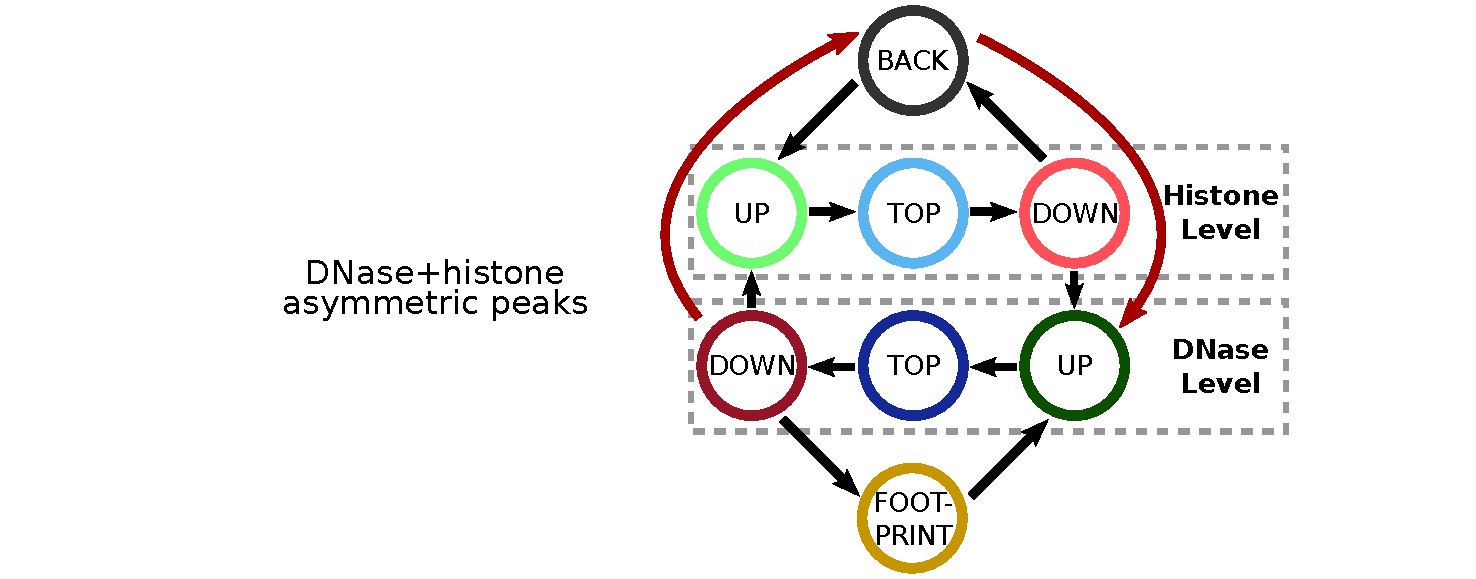
\includegraphics[width=0.99\textwidth]{gusmao_model2}
\caption[\textsc{DNase + histone asymmetric peaks model} topology]{\textbf{\textsc{DNase + histone asymmetric peaks model} topology.} Each circle represents a labeled HMM state. Each arrow represents an allowed transition between states. The red arrows represent the transitions added from the \textsc{original DNase + Histone model}. Self-transitions exist in all states and were omitted for simplicity. \emph{Source:~\cite{gusmao2014}} (modified to fit thesis format and/or clarify key points).}
\label{fig:gusmao_model2}
\end{figure}

% DNase + Histone Without Slope Model
\subsubsection{\textsc{DNase + Histone Without Slope Model}}

% Introduction
The \textsc{DNase + histone without slope model} (Figure~\ref{fig:gusmao_model3}) is a simplification of the \textsc{original DNase + Histone model}. The simplification consists on removing the slope signals and performing footprint predictions using only the normalized data. In the \textsc{DNase + histone without slope model}, the {\tt UP}, {\tt TOP} and {\tt DOWN} states from the \textsc{original DNase + histone} HMM are compressed into one state -- {\tt HIGH} -- which recognizes high levels of DNase-seq signal (DNase level state) or high levels of histone modification signal (histone level state).

% Signal
In this topology, the HMM needs only the normalized signal and becomes bivariate (DNase-seq and histone modifications normalized signals). The input matrix $\mathbf{X}$ can be represented as a vector of input signal vectors
\begin{equation}
  \label{eq:signal.m3}
  \mathbf{X} = \langle \quad \mathbf{x}^{\text{norm}}_{\text{dnase}} ,\quad \mathbf{x}^{\text{norm}}_{\text{histone}} \quad \rangle .
\end{equation}

% Figure - DNase + histone without slope model topology
\begin{figure}[h!]
\centering

\includegraphics[width=0.99\textwidth]{gusmao_model3}
\caption[\textsc{DNase + histone without slope model} topology]{\textbf{\textsc{DNase + histone without slope model} topology.}Each circle represents a labeled HMM state. Each arrow represents an allowed transition between states. The red arrows represent the transitions added from the \textsc{original DNase + Histone model}. Self-transitions exist in all states and were omitted for simplicity. \emph{Source:~\cite{gusmao2014}} (modified to fit thesis format and/or clarify key points).}
\label{fig:gusmao_model3}
\end{figure}

% DNase-only model
\subsubsection{\textsc{DNase-only Model}}

% Introduction
The \textsc{DNase-only model} (Figure~\ref{fig:gusmao_model4}) represents an alternative model to the \textsc{DNase + Histone models}. Such model uses only DNase-seq signal and the following modifications were performed in comparison to the \textsc{original DNase + Histone} HMM. The histone level states were removed and additional transitions were added: (1) from the DNase level {\tt DOWN} state to the {\tt BACK} state and (2) from the {\tt BACK} state to the DNase level {\tt UP} state.

% Signal
In this topology, the input matrix $\mathbf{X}$ can be represented as a vector of DNase-seq input signal vectors
\begin{equation}
  \label{eq:signal.m4}
  \mathbf{X} = \langle \quad \mathbf{x}^{\text{norm}}_{\text{dnase}} ,\quad \mathbf{x}^{\text{slope}}_{\text{dnase}} \quad \rangle .
\end{equation}

% Figure - DNase-only model topology
\begin{figure}[h!]
\centering
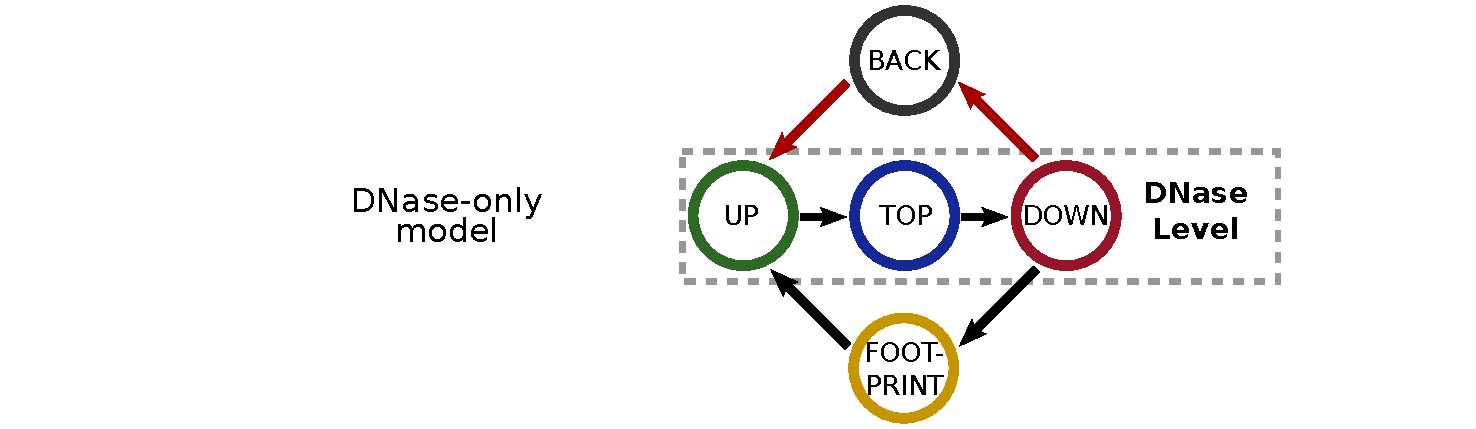
\includegraphics[width=0.99\textwidth]{gusmao_model4}
\caption[\textsc{DNase-only model} topology]{\textbf{\textsc{DNase-only model} topology.} Each circle represents a labeled HMM state. Each arrow represents an allowed transition between states. The red arrows represent the transitions added from the \textsc{original DNase + Histone model}. Self-transitions exist in all states and were omitted for simplicity. \emph{Source:~\cite{gusmao2014}} (modified to fit thesis format and/or clarify key points).}
\label{fig:gusmao_model4}
\end{figure}

% Histone-only model
\subsubsection{\textsc{Histone-only Model}}

% Introduction
The \textsc{histone-only model} (Figure~\ref{fig:gusmao_model5}) represents an alternative model to the \textsc{DNase + Histone models}. Such model uses only histone modification ChIP-seq signal. The changes in comparison to the \textsc{original DNase + histone} HMM are exactly the same as for the \textsc{DNase-only model}; however, instead of removing the histone level states, the DNase level states are removed and additional transitions are created: (1) from the histone level {\tt DOWN} state to the {\tt FOOTPRINT} state and (2) from the {\tt FOOTPRINT} state to the histone level {\tt UP} state.

% Signal
In this topology, the input matrix $\mathbf{X}$ can be represented as a vector of histone modification ChIP-seq input signal vectors
\begin{equation}
  \label{eq:signal.m5}
  \mathbf{X} = \langle \quad \mathbf{x}^{\text{norm}}_{\text{histone}} ,\quad \mathbf{x}^{\text{slope}}_{\text{histone}} \quad \rangle .
\end{equation}

% Figure - Histone-only model topology
\begin{figure}[h!]
\centering

\includegraphics[width=0.99\textwidth]{gusmao_model5}
\caption[\textsc{histone-only model} topology]{\textbf{\textsc{histone-only model} topology.} Each circle represents a labeled HMM state. Each arrow represents an allowed transition between states. The red arrows represent the transitions added from the \textsc{original DNase + Histone model}. Self-transitions exist in all states and were omitted for simplicity. \emph{Source:~\cite{gusmao2014}} (modified to fit thesis format and/or clarify key points).}
\label{fig:gusmao_model5}
\end{figure}

% Histone footprints
Unlike all aforementioned HMM topologies, the \textsc{histone-only model} generates broad footprint predictions. This stems from the fact that the histone modification ChIP-seq signals have a lower resolution than the DNase-seq signals. The \textsc{histone-only model} footprint predictions resemble, in terms of length, DNase hypersensitivity sites. The resolution difference between footprints predicted by models that use DNase-seq and models that use histone modification ChIP-seq only can be visualized in Figure~\ref{fig:gusmao_grammar_tfbs}.

%%%%%%%%%%%%%%%%%%%%%%%%%%%%%%%%%%%%%%%%%%%%%%%%%%%%%%%%%%%%%%%%%%%%%
% Section: HMM Training
%%%%%%%%%%%%%%%%%%%%%%%%%%%%%%%%%%%%%%%%%%%%%%%%%%%%%%%%%%%%%%%%%%%%%
\subsection{HMM Training}
\label{sec:hmm.training}

% Training A
We estimate the HMM parameters in a supervised manner, using the maximum likelihood method. For a given annotation sequence of the HMM states $\mathbf{q} = \langle q_1, \cdots, q_t, \cdots, q_n \rangle$ and sample data $\mathbf{X}$, the transition probabilities are estimated as
\begin{equation}
  \label{eq:hmm.train.a.1}
  a_{uv} = \frac{ \hat{a}_{uv}}{ \sum_{j=1}^{w} \hat{a}_{uj}},
\end{equation}
where $ \hat{a}_{uv} $ represents the number of transitions from state~$u$ to state~$v$ observed in the annotated training data, formally defined as
\begin{equation}
  \label{eq:hmm.train.a.2}
  \hat{a}_{uv} = \sum_{i=1}^{n-1} \mathbf{1} (q_i=u, q_{i+1}=v).
\end{equation}

% Training E
To calculate the emission probability density functions we need to estimate the Gaussian's mean ($\mu^{u}_{i}$) and covariance matrix (${\sigma}^{u}_{ik}$) for every state $u$ and input signal types $i$ and $k$. This is performed, using the maximum likelihood method, as
\begin{equation}
  \label{eq:hmm.train.e.1}
  \mu^{u}_{i} = \frac{ \sum_{j=1}^{n} {x}_{ij} {\mathbf{1}}(q_j=u) }{ \sum_{j=1}^{n} {\mathbf{1}} (q_j=u) },
\end{equation}
where $ \mu^{u}_{i} $ is the Gaussian's mean at state $u$ for the signal $i$ and
\begin{equation}
  \label{eq:hmm.train.e.2}
  {\sigma}^{u}_{ik} = \frac{\sum_{j=1}^{n} ({x}_{ij} - \mu^{u}_{i})^T({x}_{kj} - \mu^{u}_{k}) {\mathbf{1}} (q_j=u)}
  {\sum_{j=1}^{n} {\mathbf{1}} (q_j=u) - 1}.
\end{equation}
where $ \sigma^{u}_{ik} $ is the Gaussian's variance at state $u$ between signals $i$ and $k$.

% Training s
As we define the HMM to start at the {\tt BACK} state (the first HMM state), the initial transition vector $\mathbf{s}$ was manually set with the following probabilities
\begin{equation}
  \label{eq:hmm.train.s}
  \begin{array}{lcl}
    s_1 = 1 \\
    s_t = 0 \quad \forall \quad t \neq 1 \\
  \end{array}.
\end{equation}

%%%%%%%%%%%%%%%%%%%%%%%%%%%%%%%%%%%%%%%%%%%%%%%%%%%%%%%%%%%%%%%%%%%%%
% Section: HMM Decoding
%%%%%%%%%%%%%%%%%%%%%%%%%%%%%%%%%%%%%%%%%%%%%%%%%%%%%%%%%%%%%%%%%%%%%
\subsection{HMM Decoding}
\label{sec:hmm.decoding}

% Introduction
Given HMMs with topologies described in Section~\ref{sec:hmm.topology} and parameters estimated as described in Section~\ref{sec:hmm.training} we are able to perform the prediction of footprints. This prediction is performed using a well-known HMM decoding technique termed Viterbi ``algorithm''~\citep{rabiner1989}, which addresses the {\bf Problem 2} defined in Section~\ref{sec:multivariate.continuous.hmm}. Briefly, it computes the sequence of hidden states $ \mathbf{q} $ that maximizes $ p\left( \mathbf{X}, \mathbf{q} | \Theta \right) $. Then, given the computed sequence of hidden states we are able to identify the ones which corresponds to the {\tt FOOTPRINT} state. In this section we formalize the Viterbi algorithm applied in the context of computational footprinting.

% Introduction
We are interested on identifying the most probable path $ \mathbf{q^*} $ given the input $ \mathbf{X} $ on an HMM $ \Theta $. In formal terms, we are interested in evaluating the following equation
\begin{equation}
  \label{eq:viterbi1}
  \mathbf{q^*} = \argmax{\mathbf{q}} p\left(\mathbf{X}, \mathbf{q} | \Theta \right).
\end{equation}

% Exponential problem - viterbi solution
The solution to the equation~\ref{eq:viterbi1} can be found in an exaustive way by evaluating $ p\left(\mathbf{X}, \mathbf{q} | \Theta \right) $ for all $ {w}^{n} $ possible instances of the $n$-length vector $ \mathbf{q} $, in which each element assumes one of the $w$ HMM states. It is clear, however, that the complexity of such approach, in terms of the big-$\mathcal{O}$ notation is $ \mathcal{O}({w}^{n}) $, i.e. it grows exponentially given the input vector with length $n$. Fortunately, it is possible to solve the equation~\ref{eq:viterbi1} using a dynamic programming algorithm which relies on the HMM independence claims described by equations~\ref{eq:hmm.indep.1} and~\ref{eq:hmm.indep.2} with a polynomial complexity $ \mathcal{O}(n \times {w}^2) $ using the Viterbi algorithm. The Viterbi algorithm is formalized, in the context of our multivariate HMM, in the following.

% Viterbi variable
Let $ \nu_u(t) $ be a Viterbi variable, which corresponds to the probability of the most probable path of the input subset $ \langle \mathbf{{x}_{\cdot 1}}, \cdots, \mathbf{{x}_{\cdot t}} \rangle $ ending at state $ u $. Assuming knowledge of $ \nu_u(t) $, we are able to calculate the probability for the path subset $ \langle \mathbf{{x}_{\cdot 1}}, \cdots, \mathbf{{x}_{\cdot t+1}} \rangle $ using the HMM independence claims as
\begin{equation}
  \label{eq:viterbi2}
  \nu_v(t+1) = e_v(\mathbf{{x}_{\cdot t+1}}) \max_{u} \nu_u(t) a_{uv}
\end{equation}

% Viterbi algorithm - description
Let out HMM decoding start at a figurative initial time $ 0 $. We define the initial Viterbi variables for all HMM states as our initial HMM probabilities (equation~\ref{eq:hmm.initial}) as
\begin{equation}
  \label{eq:viterbi3}
  \nu_u(0) = s_u.
\end{equation}
From this initial time we are able to calculate the Viterbi variables for all the following input time points using equation~\ref{eq:viterbi2}. Furthermore, we dynamically construct a ``pointer'' vector $\boldsymbol\phi$ in which we add the most probable states in each iteration of Viterbi variable calculations for the following input time points. The algorithm is fully described as follows. In the following algorithm we denote as $ \varepsilon $ an additional figurative last state of our path $ \mathbf{q} $ in order to formally describe the algorithm termination.

\vspace{0.3cm}

% Viterbi algorithm
\begin{center}
  \begin{spacing}{1.0}
    \begin{tabular}{l}
      \hline \\[-0.25cm]
      \hspace{1.2cm} {\large {\bf \emph{ Viterbi Algorithm } } } \hspace{1.2cm} \\[0.1cm]
      \hline \\[-0.25cm]
      \hspace{0.2cm} {\bf 1. Initialization:} \\
      \hspace{0.9cm} 1.1. $ \nu_u(0) = s_u $ \\
      \hspace{0.2cm} {\bf 2. Iteration $ (t = 1, \cdots, n) $:} \\
      \hspace{0.9cm} 2.1. $ \nu_v(t) = e_v(\mathbf{{x}_{\cdot t}}) \max_{u} \nu_u(t-1)a_{uv} $ \\
      \hspace{0.9cm} 2.2. $ {\phi}_{v}(t) = \argmax{u} \nu_u(t-1) a_{uv} $ \\
      \hspace{0.2cm} {\bf 3. Termination:} \\
      \hspace{0.9cm} 3.1. $ p(\mathbf{X},\mathbf{q^*}) = \max_{u} \nu_u(n) a_{u\varepsilon} $ \\
      \hspace{0.9cm} 3.2. $ q_{n}^{\ast} = \argmax{u} \nu_u(n) a_{u\varepsilon} $ \\
      \hspace{0.2cm} {\bf 4. Reassembly $ (t = n, \cdots, 1) $:} \\
      \hspace{0.9cm} 4.1. $ q_{t-1}^{\ast} = {\phi}_{q_{t}^{\ast}}(t) $ \\[0.1cm]
      \hline
    \end{tabular}
  \end{spacing}
\end{center}

% Footprints
The footprint predictions are defined as the set of genomic intervals $F$ in which contiguous predicted hidden states $ q_t = \text{{\tt FOOTPRINT}} $. This can be written as
\begin{equation}
  \label{eq:footprint.cont}
  F = \{ f_i = [m,n] : q_t = \text{{\tt FOOTPRINT}} \quad \forall \quad m \leq t \leq n \quad \text{and} \quad q_{m-1}, q_{n+1} \neq \text{{\tt FOOTPRINT}} \}.
\end{equation}

%%%%%%%%%%%%%%%%%%%%%%%%%%%%%%%%%%%%%%%%%%%%%%%%%%%%%%%%%%%%%%%%%%%%%
% Section: Implementation
%%%%%%%%%%%%%%%%%%%%%%%%%%%%%%%%%%%%%%%%%%%%%%%%%%%%%%%%%%%%%%%%%%%%%
\section{Implementation}
\label{sec:implementation}

% HINT
We implemented our signal processing methodology and our HMM-based computational footprinting framework as a Python command line tool. Our method is called HINT -- \underline{H}MM-based \underline{I}de\underline{n}tification of \underline{T}F Footprints -- and will be referenced as such throughout this thesis. Such command line tool implements all the steps described in this chapter.

% Implementation
HINT is part of the regulatory genomics toolbox (RGT), which is a computational framework composed of a Python package and/or command line tools to handle genomic signals such as DNase-seq and ChIP-seq. The HINT tool was first released in August 2014 and is available under the terms of the GNU General Public License v3 (GPL v3). HINT python package dependencies are summarized in Table~\ref{tab:package.dependency}.

% Usage
The minimal input data required for HINT are BAM files, which is the standard file format for aligned reads for either DNase-seq or histone modification ChIP-seq. Additionally, the user may input a reference genome in order to perform the DNase-seq sequence cleavage bias correction (Section~\ref{sec:dnaseseq.sequence.cleavage.bias}). The tool outputs a BED file, which is the standard format for genomic regions (intervals). Such output BED file corresponds to the predicted footprints.

% Further information
HINT was tested on Python 2.7, Numpy 1.4.0, Scipy 0.7, Scikit-learn 0.14, Pysam 0.7.5, HMMlearn 0.0.1. We used a local Linux Ubuntu 15.04 LTS x86 $64$-bit machine running with $8$ Intel Core i7-4770 CPU at $3.40$GHz and $32$ GB RAM. Furthermore, we ran HINT on an HPC cluster mainly based on Intel Xeon-based $8$-- to $128$--way SMP $64$-bit nodes with Scientific Linux release 6.6 (Carbon).

% Table - HINT dependencies
\begin{longtable}{>{\raggedright\arraybackslash}p{2.5cm}>{\raggedright\arraybackslash}p{1.2cm}>{\raggedright\arraybackslash}p{9.8cm}}
\caption[HINT tool python package dependencies]{\textbf{HINT tool python package dependencies.}} \\
\label{tab:package.dependency} \\[-0.8cm]
  \hline
  \textbf{Package} & \textbf{Version} & \textbf{Website} \\
  \hline
  Numpy & $\geq$ 1.4.0 & \url{http://www.numpy.org/} \\
  Scipy & $\geq$ 0.7.0 & \url{http://www.scipy.org/} \\
  Scikit-learn & $\geq$ 0.14 & \url{http://scikit-learn.org/} \\
  HMMlearn & $\geq$ 0.1.1 & \url{https://github.com/hmmlearn/hmmlearn/} \\
  Pysam & $\geq$ 0.7.5 & \url{https://github.com/pysam-developers/pysam} \\
  \hline
\end{longtable}

% Website
For more information on HINT implementation please see:

\begin{center}
\url{http://www.regulatory-genomics.org/hint/}
\end{center}


%%%%%%%%%%%%%%%%%%%%%%%%%%%%%%%%%%%%%%%%%%%%%%%%%%%%%%%%%%%%%%%%%%%%%
% Section: Discussion
%%%%%%%%%%%%%%%%%%%%%%%%%%%%%%%%%%%%%%%%%%%%%%%%%%%%%%%%%%%%%%%%%%%%%
\section{Discussion}
\label{sec:discussion.3}

% Introduction
In this chapter we described our computational footprinting framework. In the first part (Section~\ref{sec:input.signal.processing}), we process the DNase-seq and histone modification ChIP-seq signals, as summarized in Figure~\ref{fig:gusmao_signal_pipeline}. In the second part (Section~\ref{sec:computational.footprinting.hmm}), we described our HMM-based approach (HINT), as summarized in Figure~\ref{fig:gusmao_method_pipeline}. Our computational footprinting framework introduced new concepts to solve the identification of active TFBS problem:

% Novel concepts
\begin{itemize}
\item We created a novel DNase-seq and histone modification ChIP-seq signal processing framework that corrects for DNase-seq sequence cleavage bias and normalizes the signal considering both within- and between-dataset signal variability. Furthermore, we applied the Savitzky-Golay smoothing filter to obtain the slope of the genomic signal.
\item We devised HMMs to segment the genome and search for the grammar of active TFBSs as shown in Section~\ref{sec:chromatin.based.method}. This novel approach is the first to integrate the full spatial profiles of both DNase-seq and histone modification ChIP-seq signal.
\item Our model is also flexible enough to consider only DNase-seq or histone modification ChIP-seq data separately. Allowing for experimental flexibility.
\item From a methodological perspective, HMMs are a favorable method choice. Window-based segmentation methods~\citep{hesselberth2009,neph2012a,piper2013} has a high dependency on footprint size definition. They rely on an extensive search using multiple window size extensions. Such methods do not take advantage of the HMM's decoding algorithms, which are able to model the length of the footprints using a probabilistic framework. Furthermore, site-centric approaches~\citep{pique2011,cuellar2012,sherwood2014,yardimci2014} do require a much higher preparation time, running time, depend highly on the model's parameters and do not necessarily fit our main goal, which is to provide a map of all putative active TFBSs for a particular cell type.
\end{itemize}


